\documentclass{article}

\usepackage[T1]{fontenc}


\usepackage{hyperref}
\usepackage{graphicx}
\usepackage[style=authoryear,backend=biber]{biblatex}
\usepackage[margin=1in]{geometry}
\usepackage[divipsnames]{xcolor}
\usepackage{float}
\usepackage{minted}
\usepackage{algorithm}
\usepackage{setspace}
\usepackage{etoolbox}
\usepackage{mathtools}
\usepackage{sourcecodepro}
\usepackage{algpseudocode}
\usepackage{mdframed}
\usepackage{pgfplots}
\usepackage{changepage}

\mdfsetup{skipabove=0pt,skipbelow=0pt}

\spaceskip=1mm

\makeatletter
\renewcommand{\ALG@name}{Pseudocode}

\bibliography{ref}

\setlength\parindent{0pt}
\setlength\parskip{0.5em}

\BeforeBeginEnvironment{minted}{\smallskip}
\AfterEndEnvironment{minted}{\smallskip}

\AtBeginEnvironment{minted}{\setstretch{1.2}}

\hypersetup{
	colorlinks = true,
	urlcolor   = blue,
	linkcolor  = blue,
	citecolor  = darkgray
}

\begin{document}

\begin{titlepage}

\centering
\vspace*{0.3cm}

\Huge
\begin{mdframed}[backgroundcolor=lightgray,linecolor=lightgray]
\centering
\vspace{7mm}
\rule{\textwidth}{2mm}

\textbf{2D \ \ Procedural \ \ Map \ \ Generation} 

\vspace{3mm}

\rule{\textwidth}{2mm}
\huge
\vfill
\
\textbf{With Pascal \& SwinGame}
\vspace{7mm}
\end{mdframed}

\vfill

\begin{tikzpicture}
\begin{axis}[
width=0.8\textwidth,
height=0.8\textwidth,
xlabel=$x$,
ylabel=$y$,
hide axis]
\addplot3[surf,
colormap/cool,
domain=0:1]
{sin(deg(8*pi*x))* exp(-20*(y-0.5)^2)
+ exp(-(x-0.5)^2*30
- (y-0.25)^2 - (x-0.5)*(y-0.25))};
\end{axis}
\end{tikzpicture}

\vfill
\large
\textbf{Jacob Milligan \\ \small Student ID - 100660682}

\end{titlepage}

\clearpage

\tableofcontents

\clearpage

\section{Procedural Generation}

\subsection{Procedural over Manual}


Very broadly speaking, in game development there are two primary ways to generate content for a project. The most common and controllable way is to produce each part by hand - in our case we'll be referring to a 2D tile map as our content.
		
For small maps this isn't a problem; it's very straight-forward to declare each tile as an element of a statically-sized 2D array (we'll go into how this is done later) and just draw those tiles 	to the screen, perhaps also drawing different sprites on top of each tile for NPC's or the player. But what happens as our map grows in size? As it goes from a $32 \times 32$ map to a $256 \times 256$ sized map, or even larger? Even if we've created a system for writing our maps out as text files to be read in, already saving lots of time, this can very quickly become time-consuming. This is a valid way of generating content, in fact the developers on CD Projekt Red's The Witcher 3: Wild Hunt did just that \parencite{witcher}, a pretty amazing feat. However, we don't have the resources or manpower of CD Projekt Red, so what's the solution?
		
\paragraph{Procedural Generation algorithms are the solution}\mbox{}
		
Games such as Minecraft, Dwarf Fortress, and the upcoming No Mans Sky all make use of procedural generation to generate enormous, beautiful, but seemingly random worlds. We say \emph{seemingly} random because, aside from computers only being able to generate \emph{pseudo}-random numbers, these algorithms are designed so that, with the same starting point, it will produce the same result.
		
\paragraph{"So then where do we start?"}
		
Good question. Many games, such as in indie title Dwarf Corp. \parencite{dwarfcorp}, begin by simulating tectonic plate activity, erosion, and river formation to carve out their terrain -  in a similar process to how terrain forms in the real world \parencite[pp. 46]{huggett}. However, we're going to go a different route and start by generating a realistic height map, a 2D array of elements that hold a generated elevation value, that we'll use to base the rest of our map off. We will use this starting point to procedurally generate a $512 \times 512$ sized map that can be navigated by the player. Along the way, we will make heavy use of the SwinGame API to handle all graphics-related functionality and briefly touch on other concepts such as basic collision detection, all of which we will code using Pascal.
	
	
\subsection{Diamonds \& Squares}


To generate a heightmap, it would be possible to design an algorithm from scratch, however that would take a long time and the result probably wouldn't be very effective, so we're going to borrow a very well-known and academically sound one called \textbf{Random Midpoint Displacement} \parencite{fournier}, also known as \textbf{the Diamond-Square Algorithm}. At its core, the purpose of this algorithm is to generate pseudo-random noise in a desirable pattern, i.e.~one that resembles a realistic spread of terrain height values. Each point of noise is stored in a data structure (in our case, a 2D array) and holds a single value - a number representing its elevation. The result is something like this:
	
\begin{figure}[H]
	\centering
	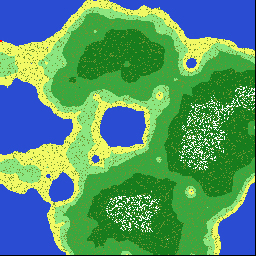
\includegraphics{map.jpg}
	\renewcommand{\figurename}{Example}
	\caption{A map generated using Diamond-Square}
\end{figure}

\paragraph{The basic concept behind Diamond-Square can be summed up like so:}
	
\begin{itemize}

	\item
		Take an empty grid which must be of size \(2^{n}+1\) in order to work. Then assign the corners a \emph{seed} value, a number that all other calculations are based off. This means that with the same seed, we should get the exact same result.
	\item
		\textbf{The Sqaure Step} - Take the grids four corners, average their total, find their mid point and assign that point the average plus a random value.
	\item
		\textbf{The Diamond Step} - Given the previous step, we now have a diamond shape surrounding a new mid point. Take the average of all points in the diamond and assign the new midpoint that value plus a random amount.
	\item
		Use a \mintinline{Pascal}{nextStep} variable to determine the next point to calculate. 
	\item
		Iterate until \mintinline{Pascal}{nextStep} is smaller than zero.
		
\end{itemize}
	
This process can be best visualized using graphs, seen in the example pictured below.
	
\begin{figure}[H]
	\centering
	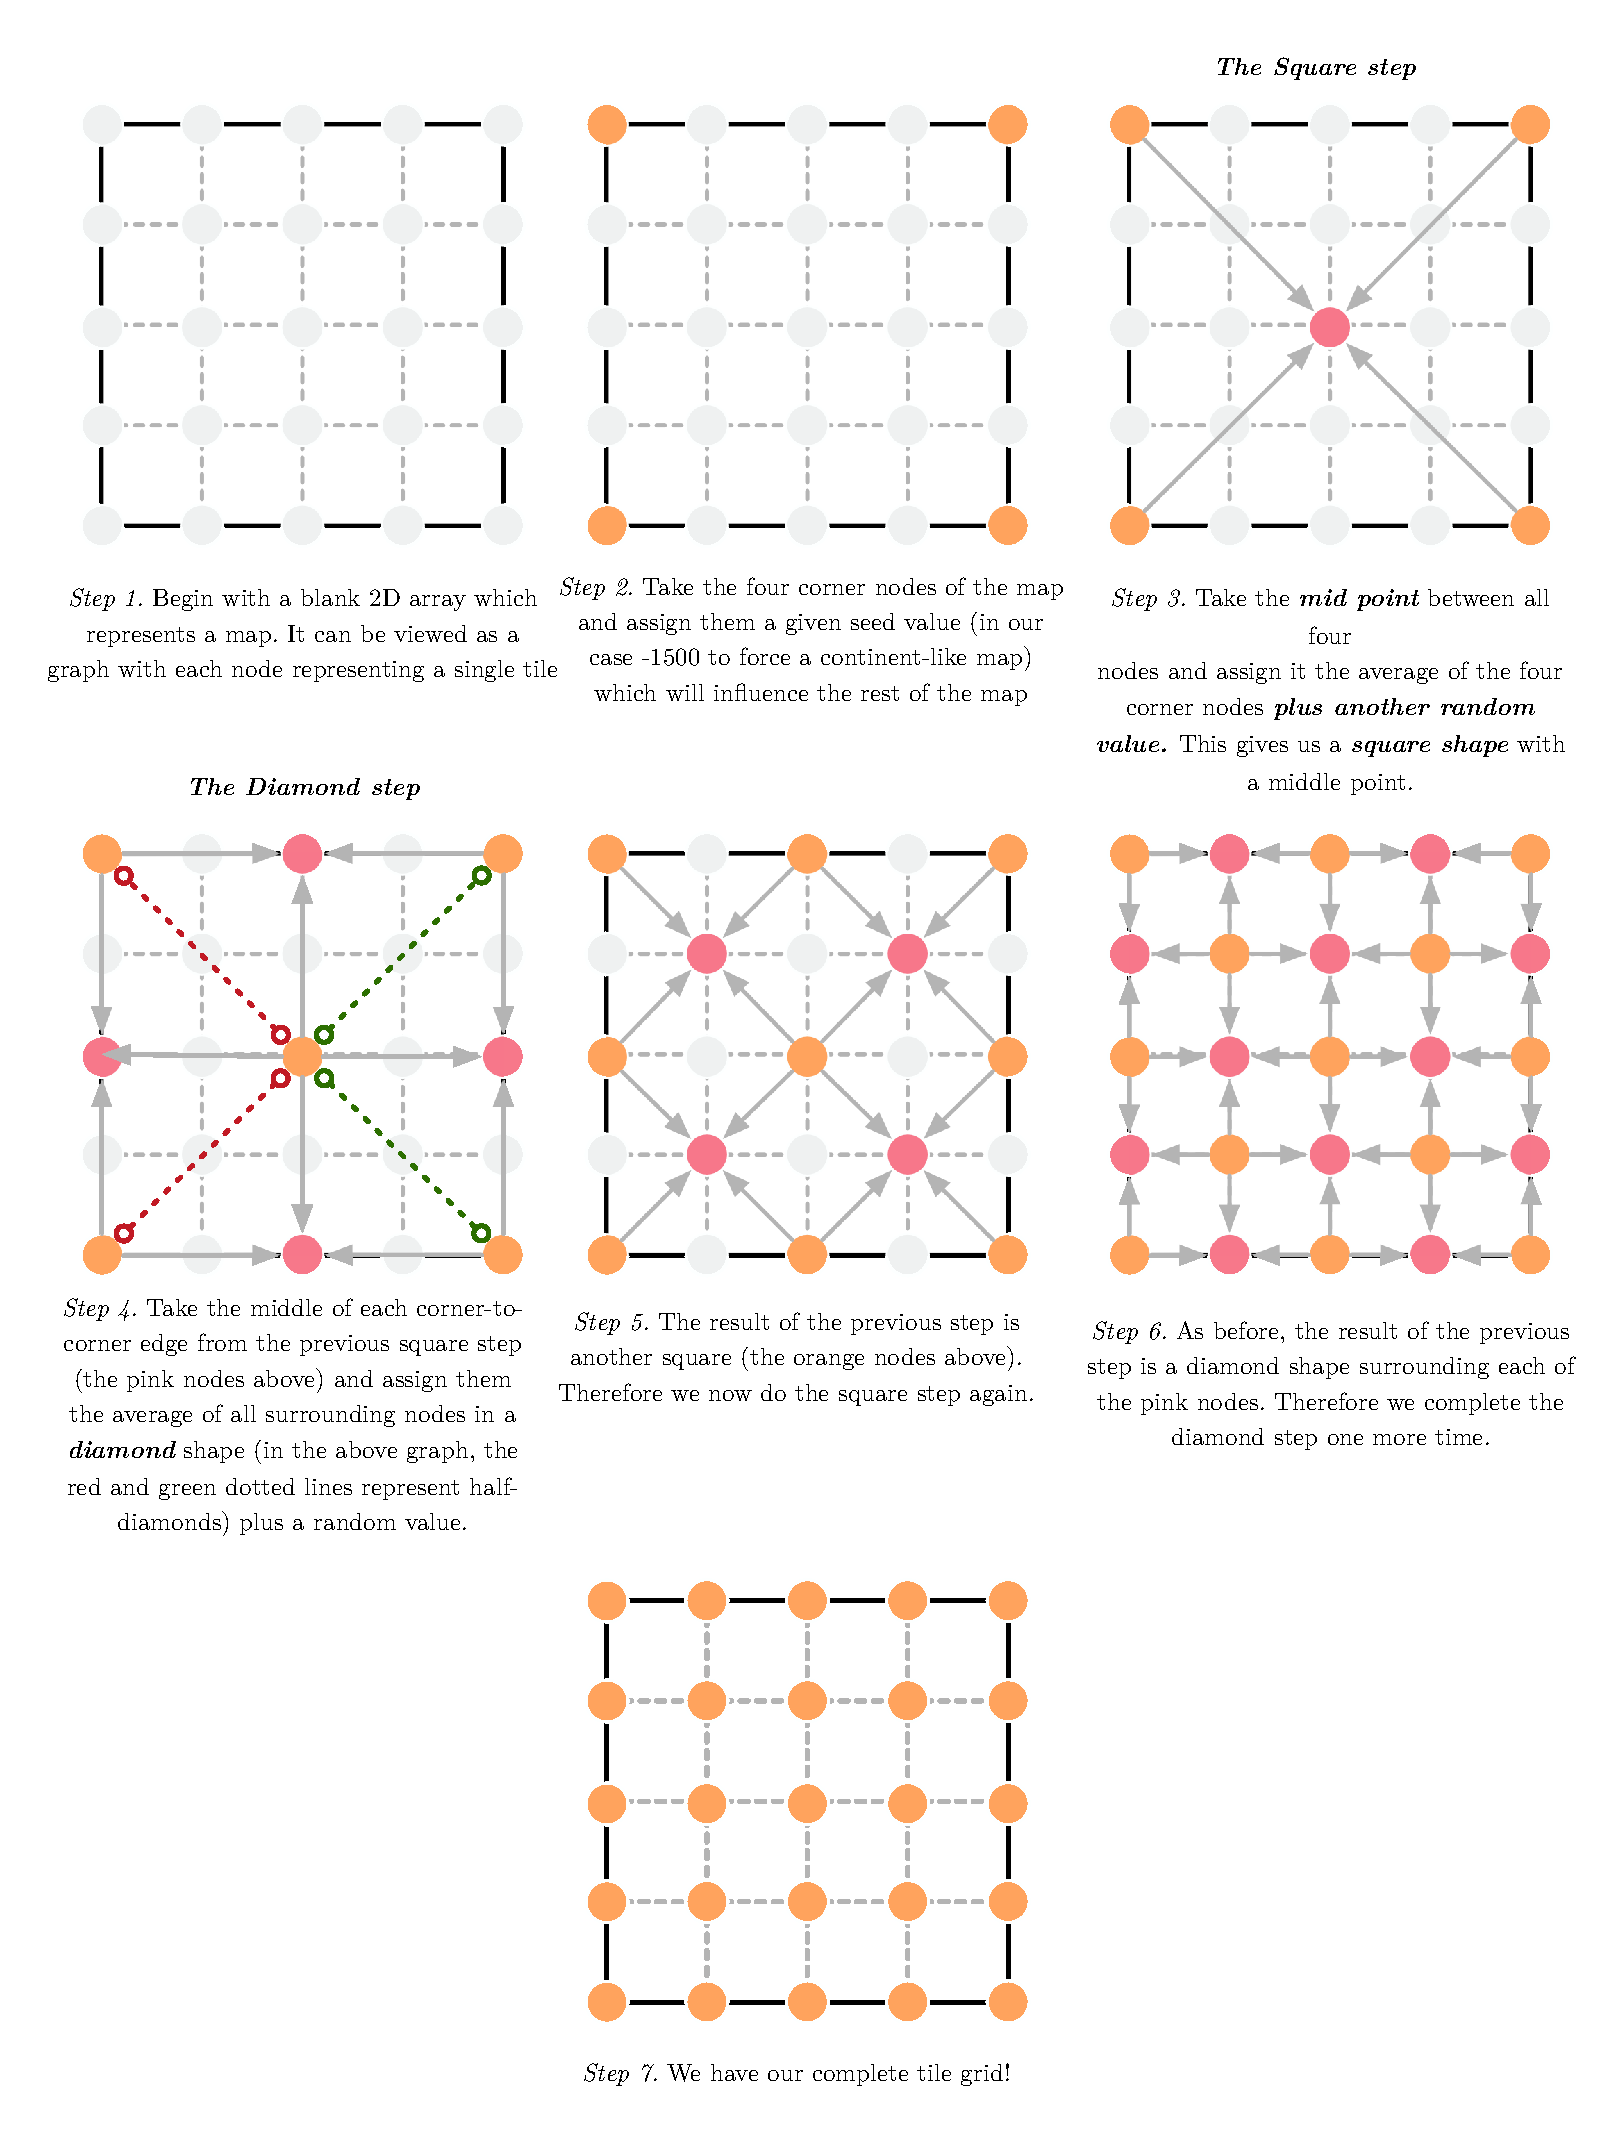
\includegraphics[width=0.9\linewidth,trim=4 4 4 4,clip]{diamondsquare.eps}
	\renewcommand{\figurename}{Example}
	\caption{Summary of the Diamond-Square algorithm}\label{fig:graph}
\end{figure}
	
\paragraph{Using this algorithm, we now have the ability to generate a starting point.}
However, before starting on an implementation, as with all software development, it's a good idea to define the requirements for our program - what functions, procedures, data structures, and features do we want to include?

We'll need the following data structures, functions, and procedures:
\begin{itemize}

\item
	First, we will define the data structures that will be required by our program. We're going to first need a \mintinline{pascal}{Tile record} to hold data related to each tile in the map such as if it's collidable, the bitmap that should be drawn for it, it's type, and elevation. We'll also need a \mintinline{pascal}{MapData record} to contain our tile grid, the players sprite and location data, and its size.
\item
	Very importantly, we'll also need our terrain generation procedures - \mintinline{pascal}{DiamondSquare()} \& \mintinline[breaklines]{pascal}{GenerateTerrain()}. \mintinline{pascal}{DiamondSquare()} will be responsible for creating a new heightmap for a passed-in \mintinline{pascal}{MapData()} record, whereas \mintinline{pascal}{GenerateTerrain()} will be responsible for deciding how each tile should be rendered based off the heightmap, alongside generating trees on the passed-in \mintinline{pascal}{MapData()} record.
\item
	Now that our terrain generation functions and structures are defined, we'll also need a \mintinline{pascal}{CreateMap()} function to call both of the above procedures and then to search for an appropriate place on the map to spawn the player.
\item
	Finally, we'll need both a \mintinline{pascal}{HandleInput()} procedure and a \mintinline{pascal}{DrawMap()} procedure to move the player around while detecting collision tiles and to draw the tile grid to the screen respectively.
	
\end{itemize}

There will also be several functions and resources referenced later on that we won't be building as they aren't directly related to procedural generation and are just utilities for allowing our map to render properly. This code sits in the \mintinline{pascal}{MapUtils.pas} file and can be downloaded from \href{https://github.com/jacobmilligan/intro_hd_report}{github}, as part of the source for the finished project, alongside the bitmap resources we'll be using (if you don't have git installed just click the 'clone or download' link and download as a zip file). These extra files are important for loading bitmaps, updating the camera position relative to the edge of the map, and drawing a map overview to the screen.


\section{Coding Terrain Generation}

\subsection{Setting Up}

\paragraph{We need to implement Diamond-Square before we can do any other terrain generation.}\mbox{}
First, download and install the \href{http://www.freepascal.org/download.var}{latest version of FPC} (Free Pascal Compiler) and a Pascal SwinGame template from the \href{http://swingame.com/index.php/downloads.html}{SwinGame Website}. Once this is complete, copy your downloaded SwinGame template to wherever you normally store your code (on my Mac it sits in \mintinline{bash}{/Users/Jacob/Dev/Repos/} - all our coding will take place in the \mintinline{bash}{/src/} folder and whenever you need to build and run the game, type the command \mintinline{bash}{./build.sh && ./run.sh} (drop the \mintinline{bash}{./} on Windows machines). Rename the \mintinline{pascal}{GameMain.pas} file to something a bit more descriptive, such as \mintinline[breaklines]{pascal}{ProceduralGeneration.pas} and open it up in your favourite text editor.

The first thing we need to do is to replace the code in the stock \mintinline{pascal}{Main()} procedure with the following:

\begin{minted}[bgcolor=darkgray,style=native]{pascal}
procedure Main();
var
  map: MapData;
begin
  DiamondSquare(map, 100, 20);
  PrintMapToConsole(map);
end;
\end{minted}

Before we render anything to a graphics window, we should first implement our algorithm and ensure that it functions correctly by printing it to the console, both procedures that will be called from \mintinline{pascal}{Main()}. We've also declared a new \mintinline{pascal}{MapData} variable which we'll be creating soon.

\vspace{1mm}

Next, create a new file in the \mintinline{bash}{/src/} directory called \mintinline{pascal}{Terrain.pas}, open it up and write a new Unit file skeleton:

\begin{mdframed}[topline=false,bottomline=false,backgroundcolor=darkgray]
\begin{minted}[style=native,tabsize=2,breaklines]{pascal}
unit Terrain;

interface
	uses SwinGame;

	type
		// Valid tile types for building maps with. Used as a terrain flag for different logic.
		TileType = (Water, Sand, Dirt, Grass, MediumGrass, HighGrass, SnowyGrass, Mountain);

		// Represents a feature on top of a tile that can have a bitmap, collision, and be interactive
		FeatureType = (NoFeature, Tree);

		// Represents a tile on the map - has a terrain flag, elevation and bitmap
		Tile = record
			flag: TileType; // Terrain type
			feature: FeatureType; // Type of feature if any
			collidable: Boolean; // Tile uses collision detection
			elevation: Integer; // The tiles elevation - zero represents sealevel.
			bmp: Bitmap; // Tiles base bitmap
			featureBmp: Bitmap; // If has feature, its bitmap
			hasBmp: Boolean;
		end;

		// Array used to hold a tilemap
		TileGrid = array of array of Tile;

		// Main representation of the current map. Holds a tile grid, alongside data related to size, smoothness, seed values.
		MapData = record
			tiles: TileGrid; // All of the tiles on a map
			player: Sprite;
			playerX, playerY: Integer; // Tile-based coordinates
			size, seed, tilesize, playerIndicator: Integer; // Map settings
		end;

	// Fills a MapData's TileGrid with generated heightmap data using the Diamond-Square fractal generation algorithm
	// This heightmap data gets used later on to generate terrain realistically
	procedure DiamondSquare(var map: MapData; maxHeight, smoothness: Integer);

	// Uses elevation values generated by DiamondSquare to assign appropriate bitmaps and randomly generate trees
	procedure GenerateTerrain(var map: MapData);
	
implementation

	procedure DiamondSquare(var map: MapData; maxHeight, smoothness: Integer);
	begin
		//code
	end;

	procedure GenerateTerrain(var map: MapData);
	begin
		//code
	end;

end.
\end{minted}
\end{mdframed}

\paragraph{That's a lot of code, so let's step through it.}\mbox{}

\begin{minted}[bgcolor=darkgray,style=native,tabsize=2,breaklines]{pascal}
unit Terrain;

interface
	uses SwinGame;

	type

		//
		//	Valid tile types for building maps with.
		//	Used as a terrain flag for different logic.
		//
		TileType = (Water, Sand, Dirt, Grass, MediumGrass, HighGrass, SnowyGrass, Mountain);

		//
		//	Represents a feature on top of a tile that can have a bitmap,
		//	collision, and be interactive
		//
		FeatureType = (NoFeature, Tree);
\end{minted}

First, we create a new \mintinline{pascal}{unit} file named \mintinline{pascal}{Terrain}. A \mintinline{pascal}{unit} file has two sections of code: 

\begin{itemize}

\item
The \mintinline{pascal}{interface} where all of our types are declared alongside \textbf{forward-declared} functions and procedures. This is the part of the \mintinline{pascal}{unit} file that other units and the main program will actually see.

\item
The  \mintinline{pascal}{implementation} section where we actually define the body of our functions and procedures.

\end{itemize}

Both of these sections of code can make use of the types, functions, and procedures created in other units through the \mintinline{pascal}{uses <UnitName>} syntax.

In the \mintinline{pascal}{type} section of the unit, we declare two enumeration types.- \mintinline{pascal}{TileType} \& \mintinline{pascal}{FeatureType}. These will be used by our \mintinline{pascal}{GenerateTerrain()} procedure and the \mintinline{pascal}{MapUtils.pas unit} file to determine how to treat different tiles. Of note is the \mintinline{pascal}{FeatureType enumeration} which at the moment can only be a Tree or nothing. Generally speaking, If we only wanted to represent Trees in the game world, we would be better off using a \mintinline{pascal}{hasTree Boolean} variable but the reason we've used an \mintinline{pascal}{enumeration} is to future-proof our program; if we wanted to, later on, add logs or rocks to the game we would only need to add a new element to \mintinline{pascal}{FeatureType} and alter the terrain generation code.

\begin{minted}[bgcolor=darkgray,style=native,tabsize=2]{pascal}
//
//	Represents a tile on the map - has a terrain flag,
//	elevation and bitmap
//
Tile = record
	// terrain type
	flag: TileType;

	// type of feature if any
	feature: FeatureType;

	// uses collision detection
	collidable: Boolean;

	//
	//	Represents the tiles elevation - zero represents sea
	//	level.
	//
	elevation: Integer;

	// tiles base bitmap
	bmp: Bitmap;

	hasBmp: Boolean;

	// bitmap for whatever feature is on top of the tiles
	featureBmp: Bitmap;
end;

//
//	Array used to hold a tilemap
//
TileGrid = array of array of Tile;

//
//	Main representation of the current map. Holds a tile grid, alongside
//	data related to size, smoothness, seed values.
//
MapData = record
	tiles: TileGrid;
	player: Sprite;
	playerX, playerY: Integer;
	size, seed, tilesize, playerIndicator: Integer;
end;
\end{minted}

\paragraph{Here, we declare our most important records and types.} The \mintinline{pascal}{Tile record} is what represents a single element of our tile grid and contains a \mintinline{pascal}{TileType} \mintinline{pascal}{flag}, a \mintinline{pascal}{FeatureType}, a \mintinline{pascal}{Boolean} variable, \mintinline{pascal}{collidable} to communicate that the particular tile is subject to collision detection, the \mintinline{pascal}{elevation Integer} value, its attached base tile \mintinline{pascal}{Bitmap} and its feature \mintinline{pascal}{Bitmap} (in this case either a Tree or an invisible bitmap) to render alongside a \mintinline{pascal}{hasBmp Boolean} value used to stop our drawing procedures from trying to draw a non-existent bitmap. We've also declared a new \mintinline{pascal}{open array of dynamic Tile arrays} to function as our tile grid. As 2D arrays are essentially just an array in which each of its elements is just another array of elements of a specified type, we've used the syntax \mintinline{pascal}{array of array of Tile} to declare this type.

\paragraph{Finally, we declare our \mintinline{pascal}{MapData} type.} This \mintinline{pascal}{record} will hold our tile grid, the players \mintinline{pascal}{Sprite} variable (A data type from the SwinGame library), the size of the map, the size of each tile, it's seed or starting value, and an indicator used by the \mintinline{pascal}{MapUtils.pas DrawMapCartography() procedure} to locate where the player is relative to the drawn tile map. Important to note is the \mintinline{pascal}{playerX} \& \mintinline{pascal}{playerY} variables as these aren't the players position in pixel coordinates (there will be a total of $275952697344$ pixels on the final map, way too large a number to even fit in a \mintinline{pascal}{LongWord} type), they are the players current pixel position translated to 2D array index equivalents - these variables will be used to calculate simple collision detection later on. Lastly, we forward declare our two terrain generation procedures.

\begin{minted}[bgcolor=darkgray,style=native,tabsize=2]{pascal}
//
//	Fills a MapData's TileGrid with generated heightmap data
//	using the Diamond-Square fractal generation algorithm
//	This heightmap data gets used later on to generate terrain realistically
//
procedure DiamondSquare(var map: MapData; maxHeight, smoothness: Integer);
	
//
//	Uses elevation values generated by DiamondSquare to assign appropriate
//	bitmaps and randomly generate trees
//
procedure GenerateTerrain(var map: MapData);
\end{minted}


\pagebreak


\subsection{Implementing Diamond-Square}

\paragraph{Moving onto the \mintinline{pascal}{implementation} section, we can now build our terrain generation algorithms.} Starting with \mintinline{pascal}{DiamondSquare}. The basic pseudocode for the algorithm looks something like this:

\begin{algorithm}[H]
\setstretch{1.35}
\caption{The Diamond-Square algorithm}
\begin{algorithmic}
\Procedure{DiamondSquare}{$map,\ maxHeight,\ smoothness$}
	\State Initialize the four corners of the map with a seed value
	\State $nextStep \gets \frac{Length(tileGrid)}{2}$
	
	\While{$nextStep > 0$}
		\ForAll{$midPoints$ of each square in the grid}  \Comment{Do square step}
			\State $midPoint \gets$ Average four corners $+ \ (Random(maxHeight) \times smoothness)$
		\EndFor
		\ForAll{Diamonds in the map} \Comment{We now have diamonds, do diamond step}
			\ForAll{$point$ in a diamond}
				\State $pointCount \gets 0$
				\If{Within boundaries of the tile grid}
					\State $midPoint \gets midPoint \ + \ point$
					\State $pointCount\gets pointCount+1$
				\EndIf
			\EndFor
			\State $midPoint \gets \frac{midPoint}{pointCount} + (Random(maxHeight) \times smoothness$)
		\EndFor
		\State $nextStep \gets \frac{nextStep}{2}$ \Comment{Smaller diamonds and squares}
		\State $smoothness \gets \frac{smoothness}{2}$ \Comment{Higher elevations have less radical difference in height}
	\EndWhile
	
\EndProcedure	
\end{algorithmic}
\end{algorithm}

When broken down like this, the process becomes a lot simpler and we have a good abstraction to reference when implementing the algorithm, so let's start on building it into our source code.

\begin{minted}[bgcolor=darkgray,style=native,tabsize=2]{pascal}
implementation

	procedure DiamondSquare(var map: MapData; maxHeight, smoothness: Integer);
	var
		x, y: Integer;
		midpointVal: Double;
		nextStep, cornerCount: Integer;
	begin
		x := 0;
		y := 0;
		midpointVal := 0;
		nextStep := Round(Length(map.tiles) / 2 ); // Center of the tile grid

		// Seed upper-left corner extremely low elevation to force it to
		// start with water
		map.tiles[x, y].elevation := -1500;
\end{minted}

Initially, we declare the x \& y variables to track our iterations through the heightmap generation process, then the \mintinline{pascal}{midpointVal Double} which we will use to calculate the current midpoint value (average plus a random value) at both the diamond and square steps. The \mintinline{pascal}{nextStep} variable is an important one and will control which tile in the grid we're analysing at any given moment and will be made smaller at each iteration until it equals 0, at which point the algorithm is finished. This is set to the centre point of the tile grid and at each iteration will be used to determine the location of a midpoint. Finally, we 'seed' the top-left corner of the map with an elevation of $-1500$ to ensure that the map will always have some ocean as its starting point which will help achieve our goal of producing a continent-like map.

\begin{minted}[bgcolor=darkgray,style=native,tabsize=2]{pascal}
// Initialize four corners of map with the same value as above
while x < Length(map.tiles) do
begin
	while y < Length(map.tiles) do
	begin
		map.tiles[x, y].elevation := map.tiles[0, 0].elevation;
		y += 2 * nextStep;
	end;

	x += 2 * nextStep;
	y := 0;
end;
\end{minted}

We then iterate all four corners of the map, stepping the entire length of the map at a time, and assign each corner the same elevation value as the top-left corner. Something that you may notice is that we aren't using the more obvious \mintinline{pascal}{for..do loop} to iterate the 2D tile grid. This is due to a quirk that's relatively unique to Pascal and some Pascal-derived languages in that a \mintinline{pascal}{for..do loop} can only increment the control variable by $1$ at a time, yet we need to increment $2 \cdot nextStep$ (currently half the size of the map) at each iteration to get to the next corner of the map, therefore we'll be using \mintinline{pascal}{while..do loops}.

\begin{minted}[bgcolor=darkgray,style=native,tabsize=2]{pascal}
x := 0;
y := 0;

while nextStep > 0 do
begin
	midpointVal := 0;
\end{minted}

Here begins the core of the generation process, essentially we want to continue to iterate the process into smaller and smaller sizes until \mintinline{pascal}{nextStep} is smaller than the size of the tile grid. Inside this loop we start with the \textbf{square step}:

\begin{minted}[bgcolor=darkgray,style=native,tabsize=2,breaklines]{pascal}
x := nextStep;
while x < Length(map.tiles) do
begin

	y := nextStep;
	while y < Length(map.tiles) do
	begin

		//
		// Sum surrounding points equidistant from the midpoint
		// in a square shape
		//
		midpointVal := map.tiles[x - nextStep, y - nextStep].elevation
					 + map.tiles[x - nextStep, y + nextStep].elevation
					 + map.tiles[x + nextStep, y - nextStep].elevation
					 + map.tiles[x + nextStep, y + nextStep].elevation;

		// Set midpoint to the average + Random value and multiply by smoothing factor
		map.tiles[x, y].elevation := Round( (midpointVal / 4) + (Random(maxHeight) * smoothness) );
		y += 2 * nextStep;
	end;

	x += 2 * nextStep;
	y := 0;
end;
\end{minted}

Here, we're scanning the tile grid for squares and their corners of the current iteration size, as in \hyperref[fig:graph]{Example 2, step 5}. \mintinline{pascal}{midpointVal} is assigned the sum of the four corners in a square surrounding the current midpoint, \mintinline[breaklines]{pascal}{map.tiles[x, y]}, then we assign the midpoints elevation the average of the points plus a random value with a maximum possible height of our passed-in \mintinline{pascal}{maxHeight} variable. Each time we do this part of the step, also seen in the diamond step, we ensure to multiply the random value by the passed-in smoothness value to allow the terrain to smooth out as the elevations become higher and the calculated map spaces become smaller. \textbf{Very importantly, because we aren't using \ \mintinline{pascal}{for..do loops}, note that we're manually resetting both \mintinline{pascal}{x} \& \mintinline{pascal}{y}}, don't forget to do this before each iteration. Let's move onto the diamond step.

\newgeometry{margin=0.5in}

\begin{minted}[bgcolor=darkgray,style=native,tabsize=2,breaklines]{pascal}
// Diamond step. Points in a diamond shape around a given midpoint. Checks if they're within the bounds of the map
x := 0;
while x < Length(map.tiles) do
begin

	y := nextStep * ( 1 - Round(x / nextStep) mod 2);
	while y < Length(map.tiles) do
	begin
		midpointVal := 0;
		cornerCount := 0;

		// Sum the surrounding points equidistant from the current midpoint in a diamond shape. Ensures that each point is within the bounds of the map
		if ( y - nextStep >= 0 ) then
		begin
			midpointVal += map.tiles[x, y - nextStep].elevation;
			cornerCount += 1;
		end;
		if ( x + nextStep < Length(map.tiles) ) then
		begin
			midpointVal += map.tiles[x + nextStep, y].elevation;
			cornerCount += 1;
		end;
		if ( y + nextStep < Length(map.tiles) ) then
		begin
			midpointVal += map.tiles[x, y + nextStep].elevation;
			cornerCount += 1;
		end;
		if ( x - nextStep >= 0 ) then
		begin
			midpointVal += map.tiles[x - nextStep, y].elevation;
			cornerCount += 1;
		end;

		// If at least one corner is within the map bounds, calculate average plus a random amount less than the map height.
		if cornerCount > 0 then
		begin
			// Set midpoint to the average of corner amt + Random value and multiply by smoothing factor
			map.tiles[x, y].elevation := Round( (midpointVal / cornerCount) + Random(maxHeight) * smoothness );
		end;

		y += 2 * nextStep;
	end;

	x += nextStep;
end;
\end{minted}

\restoregeometry

\paragraph{The diamond step is a little more complicated.} The only reason for this is that we need to do a bit more checking to ensure that a given point in the diamond is within the map boundary to avoid both calculation errors and a \mintinline{pascal}{EAccessViolation} error for accessing a non-existent memory address.

Once again we have two, nested \mintinline{pascal}{while..do loops}. Before entering each inner loop, \mintinline{pascal}{y} is assigned a new value which will be equal to the next point in the diamond. Why is this the case? Well, given the formula, where $s=$ \mintinline{pascal}{nextStep}:

\begin{equation}
y=s \cdot (1 - \left[\frac{x}{s} \ mod \ 2\right]
\end{equation}

If we were to plug in $x=0$ \& $s=3$ which is where $x$ will start at the beginning of the diamond step and what \mintinline{pascal}{nextStep} will be set to in the first iteration of a $5 \times 5$ grid, we would get:

\begin{equation}
\begin{split}
y&=3 \cdot (1 - \left[\frac{0}{3} \ mod \ 2\right]) \\
&=3 \cdot (1 - \left[0 \ mod \ 2\right]) \\
&=3 \cdot (1 - [0]) \\
&=3
\end{split}
\end{equation}

\mintinline{pascal}{y} is now the right point of the diamond, then, given \mintinline{pascal}{x += nextStep} in the next iteration, \mintinline{pascal}{x} will now be $3$, so if we plug that into the formula again, we get:

\begin{equation}
\begin{split}
y&=3 \cdot (1 - \left[\frac{3}{3} \ mod \ 2\right]) \\
&=3 \cdot (1 - \left[1 \ mod \ 2\right]) \\
&=3 \cdot (1 - [1]) \\
&=3 \cdot 0 \\
&=0
\end{split}
\end{equation}

So now \mintinline{pascal}{y} is set to the top point of the diamond and so on. This simple formula allows us to iterate four points of a diamond without having to resort to using \mintinline{pascal}{if} statements.

In the body of the inner loop, we then check each point surrounding the mid-point to see if it's inside the bounds of the map. If it is, we increment \mintinline{pascal}{cornerCount} once. Then, after checking all points we assign the mid-point the average of all surrounding points within the bounds of the map plus a random value limited to our \mintinline{pascal}{maxHeight} variable multiplied by the current smoothness factor. Finally, we increase the value of \mintinline{pascal}{y} in the inner loop by the length of the current diamond to get the lower point and iterate until all diamonds in the current loop are calculated.

\begin{minted}[bgcolor=darkgray,style=native,tabsize=2,breaklines]{pascal}
		nextStep := Round(nextStep / 2); // Make the next space smaller

		//
		//	Increase smoothness for every iteration, allowing
		//	less difference in height the more iterations that are completed
		//
		smoothness := Round(smoothness / 2);
	end;
end;
\end{minted}

\paragraph{We're almost done.} At the end of the current diamond-square iteration, we make the size of our diamonds and squares smaller by halving \mintinline{pascal}{nextStep} alongside halving \mintinline{pascal}{smoothness} so that higher elevations have a less radical difference in height. Changing our smoothness value is what creates a realistic gradient in heights and a more visually pleasing result.

\subsection{Testing}

\paragraph{The most complex and difficult part is out of the way.}But before we do anything else, we need to test it. If we were to wait until we had all of our drawing, collision, and update functions coded up, we'd be well into finishing our program before we've even made sure the core algorithm behind it even works! To do this, we can go back to our main program file, \mintinline{pascal}{ProceduralGeneration.pas}, and implement the \mintinline[breaklines]{pascal}{PrintMapToConsole()} and \mintinline[breaklines]{pascal}{CreateMap()} procedures/functions we wrote in \mintinline{pascal}{Main()}.

\begin{minted}[bgcolor=darkgray,style=native,tabsize=2,breaklines]{pascal}
// Prints all of the elevation data in a tilemap to the console.
// Don't use for maps larger than 16 x 16 or it will be bigger than the console window
procedure PrintMapToConsole(constref map: MapData);
var
	x, y: Integer;
begin
	for x := 0 to High(map.tiles) do
  	begin
  		for y := 0 to High(map.tiles) do
	  	begin
  			Write(map.tiles[x, y].elevation, ' ');
	  	end;
  		WriteLn();
	  end;
end;
\end{minted}

The code for this function is fairly self-explanatory - we iterate the 2D array and write all \mintinline[breaklines]{pascal}{y} values without appending a newline, then at the end of each \mintinline[breaklines]{pascal}{x} iteration, write a newline to the console to simulate a grid. 

\begin{minted}[bgcolor=darkgray,style=native,tabsize=2,breaklines]{pascal}
//
//  Initializes a new tile grid and then generates a new map using DiamondSquare().
//  The new map can be random or based off a given seed
//
function CreateMap(size: Integer; random: Boolean; seed: Integer = 0): MapData;
var
  i, j: Integer;
begin
  result.tilesize := 32;
  result.size := size;
  result.player := CreateSprite('player', BitmapNamed('player')); // We'll use this later

  // Setup seed
  if random then
  begin
    Randomize;
  end
  else
  begin
    RandSeed := seed;
  end;

  // Initialize Tile Grid
  SetGridLength(result.tiles, size);
  // Generate Heightmap
  DiamondSquare(result, 100, 20);
end;
\end{minted}

\mintinline[breaklines]{pascal}{CreateMap()} takes three parameters - a value to determine the map size, a \mintinline[breaklines]{pascal}{Boolean} variable to determine if we should generate a random map or one from a pre-determined seed value, We first assign a tilesize, size, and sprite for our \mintinline[breaklines]{pascal}{MapData result} variable. Then, if \mintinline[breaklines]{pascal}{random} is true we call the \mintinline[breaklines]{pascal}{Randomize procedure} which initializes Pascals internal random number generator with a new, unique seed to base all random generation off. Much like our \emph{seed} value used to base all of our Diamond-Square calculations off, the Pascal \mintinline[breaklines]{pascal}{Random()} function, a deterministic \emph{pseudo-random} number generation algorithm, itself requires a seed value, generated by the exact time on the computers system clock down to nanoseconds, to base its calculations off. If \mintinline[breaklines]{pascal}{random} is false, we then assign our seed value to the Pascal \mintinline[breaklines]{pascal}{RandSeed} variable, which sets \mintinline[breaklines]{pascal}{Random()}'s seed value manually. We then call \mintinline[breaklines]{pascal}{SetGridLength()} (listed below) to initialize our 2D array and pass our map into \mintinline[breaklines]{pascal}{DiamondSquare()} to get assigned a heightmap.

\begin{minted}[bgcolor=darkgray,style=native,tabsize=2,breaklines]{pascal}
//	Initializes the 2D map grid with the given size and sets the default 
//	values for each tile
procedure SetGridLength(var tiles: TileGrid; size: Integer);
var
	column: Integer;
	x, y: Integer;
begin

	// Set all of the column sizes to the right length
	for column := 0 to size do
	begin
		SetLength(tiles, column, size);
	end;

	// Iterate map and setup default values for all tiles
	for x := 0 to High(tiles) do
	begin
		for y := 0 to High(tiles) do
		begin
			// Setup default values
			tiles[x, y].elevation := 0;
			tiles[x, y].collidable := false;
			tiles[x, y].feature := NoFeature;
			tiles[x, y].hasBmp := false;
		end;
	end;
end;
\end{minted}

Now that we have all of our core procedures and functions defined, we can test out our \mintinline[breaklines]{pascal}{DiamondSquare() procedure} by calling \mintinline[breaklines]{pascal}{CreateMap(9, 100, 20)} from \mintinline[breaklines]{pascal}{Main()}; we want to pass in a very small size value to \mintinline[breaklines]{pascal}{CreateMap()} otherwise we won't be able to see all of the printed elevation numbers in the console. Note that we're passing in a size of $9$ rather than $8$; this is because, as previously discussed, \mintinline[breaklines]{pascal}{DiamondSquare()} only works for sizes equivalent to $2^{n}+1$. Run \mintinline[breaklines]{bash}{./build.sh && ./run.sh} in the console from the root project folder and we can see the result:

\begin{figure}[H]
	\centering
	\renewcommand{\figurename}{Example}
	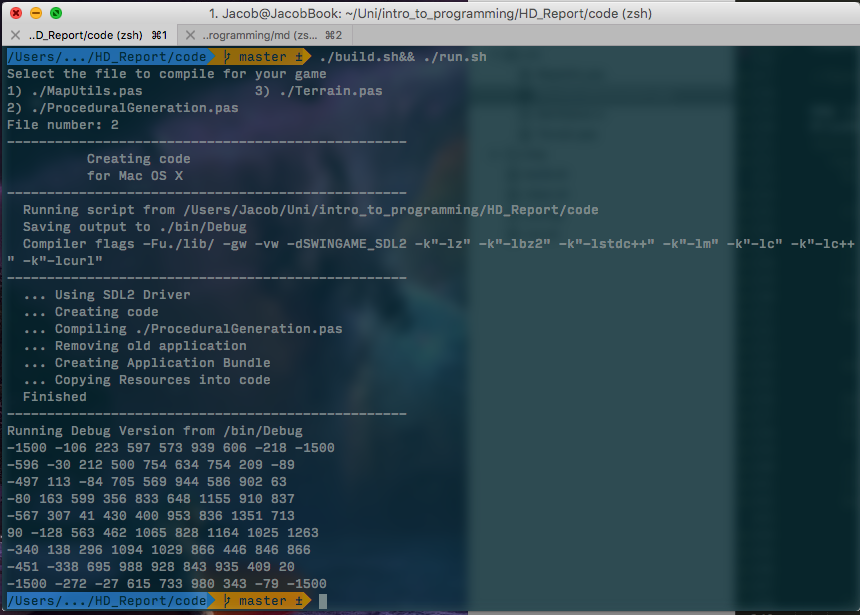
\includegraphics[width=0.9\linewidth,trim=4 4 4 4,clip]{printtoconsole.png}
	\caption{The heightmap printed to the console}
\end{figure}

It works! It may look fairly unimpressive now but at least we can verify that our algorithm works and produces pseudo-random values across a nice, smooth gradient. Let's move onto our \mintinline[breaklines]{pascal}{GenerateTerrain()} procedure to actually begin implementing a graphical representation of our map.

\subsection{Generating Terrain and Features}

\paragraph{In order to graphically represent terrain, we need to assign Bitmaps and \mintinline[breaklines]{pascal}{FeatureTypes}.} This will be defined in our \mintinline[breaklines]{pascal}{GenerateTerrain() procedure}. This step in terrain generation is less complex than \mintinline[breaklines]{pascal}{DiamondSquare()} \emph{at the present}; it's possible, and encouraged, to extend this this procedure after finishing the program and, for many procedurally generated games, \mintinline[breaklines]{pascal}{DiamondSquare()} is just the beginning and their most complex algorithms belong in the terrain generation procedures and functions. However, our focus is on generating a base world to get started with procedural generation, but if you are interested I would recommend visiting the Procedural Content Generation Wiki \parencite{pcg} and browsing the many articles listed there.

Before we dive into coding our \mintinline[breaklines]{pascal}{GenerateTerrain() procedure} lets outline exactly how we want it to work by using abstraction through pseudocode.

\begin{algorithm}[H]
\setstretch{1.35}
\caption{Procedure to Generate Terrain}
\begin{algorithmic}
\Procedure{GenerateTerrain}{$map$}
	\For{$x \gets 0$ \ To \ $High(tiles)$} \Comment{Generate tile Bitmaps}
		\For{$y \gets 0$ \ To \ $High(tiles)$}
			\State Assign a different Bitmap to $tiles[x, y]$ for different $elevation$ ranges
			\If{$tiles[x,y]$ $elevation$ value is $< 0$}
				\State $tiles[x, y] \gets$ Dark Water Bitmap
			\Else
				\State $tiles[x, y] \gets$ Mountain Bitmap \Comment{$elevation > 1499$}
			\EndIf
			
			\If{$Random() > 0.9$ \textbf{and} $tiles[x,y]$ is not a Water tile}
				\State $tiles[x, y]'s \ FeatureType \gets$ A tree appropriate for the current tile type
			\EndIf
		\EndFor
	\EndFor
\EndProcedure	
\end{algorithmic}
\end{algorithm}

Essentially all we need to do is iterate over our entire 2D heightmap and assign each tile a Bitmap based on its elevation value. At certain elevations we may choose to apply different processes later on, but all we're doing at the moment is assigning the right tile Bitmap to the right elevation value. The second part of the process is generating appropriate tree Bitmaps based on a very random process; it's highly encouraged to extend this and explore \label{forestalgo}forest generation algorithms that work by creating seeds, sunlight, and maturation processes (see \cite{forests}) but for the moment we're going to apply a process to achieve a semi-procedural result.

\begin{minted}[bgcolor=darkgray,style=native,tabsize=2,breaklines]{pascal}
// Generates the terrain type for each tile based off its elevation value
procedure GenerateTerrain(var map: MapData);
var
	x, y: Integer;
begin
	// Iterate all tiles and change their bitmap and data depending on their
	// pre-generated altitude
	for x := 0 to High(map.tiles) do
	begin
		for y := 0 to High(map.tiles) do
		begin

			// Setup the tiles
			case map.tiles[x, y].elevation of
				0..199: SetTile(map.tiles[x, y], Water, 'water', true);
				200..299: SetTile(map.tiles[x, y], Sand, 'sand', false);
				300..399: SetTile(map.tiles[x, y], Grass, 'grass', false);
				400..599: SetTile(map.tiles[x, y], MediumGrass, 'dark grass', false);
				600..799: SetTile(map.tiles[x, y], HighGrass, 'darkest grass', false);
				800..999: if Random(10) > 6 then
							// Generate patchy snow at mid-to-high elevations
							SetTile(map.tiles[x, y], SnowyGrass, 'snowy grass', false)
						  else
							SetTile(map.tiles[x, y], HighGrass, 'darkest grass', false);
				1000..1499: SetTile(map.tiles[x, y], SnowyGrass, 'snowy grass', false);
\end{minted}

First, we delare our \mintinline[breaklines]{pascal}{GenerateTerrain()} procedure and begin iterating the 2D tile grid. We then define several elevation ranges inside a \mintinline[breaklines]{pascal}{case} statement for which we assign the current tiles Bitmap using \mintinline[breaklines]{pascal}{SetTile()} (which we'll implement soon) - lower elevation get water, while higher elevations get snowy grass. At elevation ranges of $800-999$ we randomly assign either snow or grass to simulate patchy snow as the terrain transitions to higher elevation values.

\begin{minted}[bgcolor=darkgray,style=native,tabsize=2,breaklines]{pascal}
				else
					// Only generate dark water if elevation is low enough
					// otherwise, every other value, which will be higher than 1499, should
					// become mountains
					if map.tiles[x, y].elevation  < 0 then
						SetTile(map.tiles[x, y], Water, 'dark water', true)
					else
						SetTile(map.tiles[x, y], Mountain, 'mountain', true)
			end;

			// Generates trees randomly. Feel free to extend this by making your own
			// procedural tree generation algorithm to make beautiful forests!
			if ( Random() > 0.9 ) and ( map.tiles[x, y].flag <> Water ) then
			begin
				SetFeature(map.tiles[x, y], Tree, true);
			end;

		end;
	end;
end;
\end{minted}

If the current tiles elevation value is outside the specified ranges we fall to the \mintinline[breaklines]{pascal}{else} block and assign elevations lower than $0$ deep water tiles, otherwise anything not less than $0$ must be higher than $1499$ so we assign it a mountain tile. Finally, we randomly set the tiles \mintinline[breaklines]{pascal}{featureBmp} to either a tree or nothing depending on a random value and as long as the tile isn't water - trees don't generally grow in the ocean.

\paragraph{You will have noticed both \mintinline[breaklines]{pascal}{SetTile()} \& \mintinline[breaklines]{pascal}{SetFeature()} procedures.} These handle assigning default values to tiles and assigning the right tree for the right \mintinline[breaklines]{pascal}{TileType} respectively. Let's quickly code them up:

\begin{minted}[bgcolor=darkgray,style=native,tabsize=2,breaklines]{pascal}
// Sets a tiles values to specified. Anything with collidable set to true
// won't be able to be walked over by the player
procedure SetTile(var newTile: Tile; flag: TileType; bmp: String; collidable: Boolean);
begin
	newTile.flag := flag;
	newTile.bmp := BitmapNamed(bmp);
	newTile.collidable := collidable;
	newTile.hasBmp := true;
end;
\end{minted}

\mintinline[breaklines]{pascal}{SetTile()} assigns all of the specified values alongside any required default values for a given tile which saves us the hassle of rewriting this code each time we want to setup a tile.

\begin{minted}[bgcolor=darkgray,style=native,tabsize=2,breaklines]{pascal}
//
//	Sets up a new feature on a given tile. At the moment we only have trees
//	as valid features but it's really easy for you to add more features! 
//	Why not try adding rocks, logs or even treasure?
//
procedure SetFeature(var tile: Tile; feature: FeatureType; collidable: Boolean);
begin
	tile.feature := feature;
	tile.collidable := collidable;

	if feature = Tree then
	begin
		case tile.flag of
			Water: tile.featureBmp := BitmapNamed('hidden');
			Sand: tile.featureBmp := BitmapNamed('palm tree');
			Dirt: tile.featureBmp := BitmapNamed('tree');
			Grass: tile.featureBmp := BitmapNamed('tree');
			MediumGrass: tile.featureBmp := BitmapNamed('pine tree');
			HighGrass: tile.featureBmp := BitmapNamed('pine tree');
			SnowyGrass: tile.featureBmp := BitmapNamed('snowy tree');
			Mountain: tile.featureBmp := BitmapNamed('hidden');
		end;
	end;
end;
\end{minted}

\mintinline[breaklines]{pascal}{SetFeature()} is fairly self explanatory - it uses a \mintinline[breaklines]{pascal}{case} statement on the passed-in tiles \mintinline[breaklines]{pascal}{TileType} to determine which tree bitmap to load up. Notice, a feature can be collidable (you shouldn't be able to walk through trees) and, using the syntax \mintinline[breaklines]{pascal}{if feature = <FeatureType> then}, we can specify different logic for different types of features, once again future-proofing our program for extensibility.

\paragraph{Return to \mintinline[breaklines]{pascal}{CreateMap()}} and add in a call to \mintinline[breaklines]{pascal}{GenerateTerrain(result)}. If you run the program now, the program won't work. In order to draw the map to the screen, we need to both load our resources up and implement a \mintinline[breaklines]{pascal}{DrawMap()} procedure.

\section{Drawing, Input, and Collision}

\subsection{Drawing the map}

Before we can draw anything to the screen we need to open a SwinGame graphics window and define a main game loop, so let's go to our \mintinline[breaklines]{pascal}{Main()} procedure and edit to look like this:

\begin{minted}[bgcolor=darkgray,style=native,tabsize=2,breaklines]{pascal}
procedure Main();
var
  map: MapData;
begin

  LoadResources();
  
  // Open a SwinGame graphics window for drawing to
  OpenGraphicsWindow('Procedural Map Generation', 800, 600);
  
  map := CreateMap(513, true);

  repeat
    ProcessEvents();

    ClearScreen(ColorBlack);
    
    UpdateCamera(map);
    DrawMap(map);
    DrawSprite(map.player);

    RefreshScreen(60);
  until WindowCloseRequested();
end;
\end{minted}

We define our main game loop to \mintinline[breaklines]{pascal}{repeat..until WindowCloseRequested()}, which happens when the user exits the window. Both \mintinline[breaklines]{pascal}{LoadResources()} \& \mintinline[breaklines]{pascal}{UpdateCamera()} are from the \mintinline[breaklines]{pascal}{MapUtils.pas unit} file and do exactly what the say they do, loading resources and making sure the camera is always centered on our player. We call \mintinline[breaklines]{pascal}{DrawMap()} to draw our map to the screen, the procedure we'll be implementing, and the SwinGame API's \mintinline[breaklines]{pascal}{DrawSprite()} procedure to draw the player to the screen. \mintinline[breaklines]{pascal}{ClearScreen()} \& \mintinline[breaklines]{pascal}{RefreshScreen()} are called every iteration alongside \mintinline[breaklines]{pascal}{ProcessEvents()} for input handling.

\paragraph{Before we implement \mintinline[breaklines]{pascal}{DrawMap()}, we need to create a function to check if a particular element is inside the bounds of the tile grid.} \

\begin{mdframed}[backgroundcolor=darkgray]
\begin{minted}[style=native,tabsize=2,breaklines]{pascal}
//
//	Determines whether a given point is inside the tilemap or not
//
function IsInMap(constref map: MapData; x, y: Integer): Boolean;
begin
	result := false;

	// Check map bounds. As every map is (2^n)+1 in size, the bounds
	// stop at High()-1 which will be a number equal to 2^n.
	if (x > 0) and (x < High(map.tiles) - 1) and (y > 0) and (y < High(map.tiles) - 1) then
	begin
		result := true;
	end;
end;
\end{minted}
\end{mdframed}

\paragraph{Once we've implemented \mintinline[breaklines]{pascal}{IsInMap()} we can move onto \mintinline[breaklines]{pascal}{DrawMap()}:} 
\
\vspace{0.5cm}

\begin{mdframed}[backgroundcolor=darkgray]
\begin{minted}[style=native,tabsize=2,breaklines]{pascal}
//
//	Draws the current map data to the screen but only within the bounds of
//	the current Camera view.
//
procedure DrawMap(constref map: MapData);
var
	x, y: Integer;
	newView: TileView;
begin
	// Get a new tile view to see what should be drawn
	newView := CreateTileView(map);

	// Iterate only tiles in the tile map that correspond to a
	// visible tile 
	for x := newView.x to newView.right do
  	begin
	  	for y := newView.y to newView.bottom do
	  	begin
	  		
	  		if IsInMap(map, x, y) and map.tiles[x, y].hasBmp then
	  		begin
	  			// Draw the tile
	  			DrawBitmap(map.tiles[x, y].bmp, x * map.tilesize, y * map.tilesize);
	  			// Draw a tree or no feature
					DrawBitmap(map.tiles[x, y].featureBmp, x * map.tilesize, y * map.tilesize);
	  		end;

	  	end;
  	end;
end;
\end{minted}
\end{mdframed}

\

In our \mintinline[breaklines]{pascal}{DrawMap()} procedure we create a new \mintinline[breaklines]{pascal}{TileView} record, this is from the \mintinline[breaklines]{bash}{MapUtils.pas} unit file and is used to translate the current camera view in pixels ($800 \times 600$ in the case of our game) into tile grid coordiantes ($25 \times 19$). We then make use of the \mintinline[breaklines]{pascal}{x, right, y, bottom record} members it returns to draw whatever tiles are currently within the cameras view to the screen through a nested \mintinline[breaklines]{pascal}{for..do} loop, ensuring that the tile is inside the map bounds and has an assigned bitmap before drawing it. It's important when creating large maps to ensure that only the tiles that are visible are drawn to the screen - if we were drawing $512 \cdot 512 = 262,144$ tiles to the screen at each game loop, the program would run extremely slow.
 
\subsection{Handling Input}
\paragraph{Now that we've implemented our drawing procedure, let's move onto input and collision detection:}

 
 \vspace{0.5cm}
 \
 \begin{mdframed}[backgroundcolor=darkgray]
 \begin{minted}[style=native,tabsize=2,breaklines]{pascal}
procedure HandleInput(var map: MapData);
var
	newX, newY: Integer;
begin

	// Used to determine if they should be allowed to move in a given direction
	newX := map.playerX;
	newY := map.playerY;

	// Change values depending on direction
	if KeyDown(UpKey) then
	begin
		newY -= 1;
	end;
	if KeyDown(RightKey) then
	begin
		newX += 1;
	end;
	if KeyDown(DownKey) then
	begin
		newY += 1;
	end;
	if KeyDown(LeftKey) then
	begin
		newX -= 1;
	end;
 \end{minted}
 \end{mdframed}
 \
 
Here, we pass in our \mintinline[breaklines]{pascal}{MapData} variable and save the players current tile grid based $x$ and $y$ values with \mintinline[breaklines]{pascal}{newX} \& \mintinline[breaklines]{pascal}{newY} because we'll be altering this data later. Next we use the SwinGame procedure \mintinline[breaklines]{pascal}{KeyDown()} to move the players $x$ \& $y$ values in the right direction. Essentially we're \emph{predicting} what the players coordinates will be on the next iteration of the game loop before we \emph{actually} move the player, which is why we aren't assigning these new coordinates to the player directly, rather saving the predicted coordinates in order to do some collision detection:
 
 \clearpage
 
 \begin{mdframed}[backgroundcolor=darkgray]
 \begin{minted}[style=native,tabsize=2,breaklines]{pascal}
	//	If either newX or newY are outside the map bounds or are a collidable tile, reset
	//	the players position and don't move them
	if (newX <= 0) or (newX >= High(map.tiles) - 1) or (map.tiles[newX, newY].collidable) then
	begin
		newX := map.playerX;
	end;
	if (newY <= 0) or (newY >= High(map.tiles) - 1) or (map.tiles[newX, newY].collidable) then
	begin
		newY := map.playerY;
	end;

	// Assign the new values to the player
	map.playerY := newY;
	map.playerX := newX;

	// Move the player according to world coordinates rather than tile
	// coordinates by multiplying their tile coordinates by the tilesize
	SpriteSetY(map.player, map.playerY * map.tilesize);
	SpriteSetX(map.player, map.playerX * map.tilesize);

end;
 \end{minted}
 \end{mdframed}

\

In the above \mintinline[breaklines]{pascal}{if..then} statements we check to see if the players predicted $x$ or $y$ values are outside the map bounds or are on top of a collidable tile. If either of these conditions are true, then we reset either one or both axis' by assigning \mintinline[breaklines]{pascal}{newX or newY} the players original coordinate values. Finally, we assign the new tile-based coordinates, whether they've changed or not, to the player directly and call the SwinGame \mintinline[breaklines]{pascal}{SpriteSetX()} \& \mintinline[breaklines]{pascal}{SpriteSetY()} procedures to actually change the players in-game pixel-based coordinates by multiplying the tile values by the maps \mintinline[breaklines]{pascal}{tilesize} value.

\subsection{Finishing Up}

\paragraph{We're almost done.} However, first we need to append our \mintinline[breaklines]{pascal}{Main()} \& \mintinline[breaklines]{pascal}{CreateMap()} procedures with some new code to allow our player to spawn in a correct location and to handle input.
\
Edit \mintinline[breaklines]{pascal}{CreateMap()} with the following code:
\
\vspace{0.5cm}

\begin{adjustwidth}{-1.5cm}{-1.5cm}
\begin{mdframed}[backgroundcolor=darkgray]
\begin{minted}[style=native,tabsize=2,breaklines]{pascal}
//	Initializes a new tile grid and then generates a new map using DiamondSquare().
//	The new map can be random or based off a given seed
function CreateMap(size: Integer; random: Boolean; seed: Integer = 0): MapData;
var
	i, j: Integer;
	spawnFound: Boolean;
begin
	result.tilesize := 32;
	result.size := size;
	result.player := CreateSprite('player', BitmapNamed('player'));

	// Setup seed
	if random then
	begin
		Randomize;
	end
	else
	begin
		RandSeed := seed;
	end;

	// Initialize Tile Grid
	SetGridLength(result.tiles, size);
	// Generate Heightmap
	DiamondSquare(result, 100, 20);

	GenerateTerrain(result);

	//	Search for the first sand tile without a feature on it, thus spawning the player on a beach
	spawnFound := false;
	for i := 0 to High(result.tiles) do
	begin
		if spawnFound then
			break;

		for j := 0 to High(result.tiles) do
		begin
			if spawnFound then
				break;

			// Search for a sand tile to spawn the player on
			if (i > 1) and (result.tiles[i, j].flag = Sand) and (result.tiles[i, j].feature = NoFeature) then
			begin
				SpriteSetX(result.player, i * 32);
				SpriteSetY(result.player, j * 32);
				result.playerX := i;
				result.playerY := j;
				spawnFound := true;
			end;
		end;
	end;

	// Recursively call self with new random value if spawn not found
	if not spawnFound then
	begin
		CreateMap(size, true, seed);
	end;
end;
\end{minted}
\end{mdframed}
\end{adjustwidth}

\paragraph{The primary addition here, is to search for the players spawn point.} We create a nested \mintinline[breaklines]{pascal}{for..do} loop to iterate the tile grid and search for the first sand tile, then assign the players position accordingly; a very simple way to find a spawn point but effective enough for our program. The most interesting section of code in this procedure is also the shortest:

\begin{minted}[bgcolor=darkgray,style=native,tabsize=2,breaklines]{pascal}
// Recursively call self with new random value if spawn not found
if not spawnFound then
begin
	CreateMap(size, true, seed);
end;
\end{minted}

If the specified seed or random seed value produces a map with only water tiles then we use \textbf{recursion} to call \mintinline[breaklines]{pascal}{CreateMap()} itself again but with a new random seed. The idea of recursion in programming occurrs when part of a procedure or function calls itself and runs the same block of code again, often with new parameters; the return value of which follows the chain of recursion back to the start, itself being recursive by definition \parencite{recursion}. This means that the \mintinline[breaklines]{pascal}{CreateMap()} procedure will keep calling itself until it produces a valid map with a valid spawn point.

\paragraph{Finally, edit \mintinline[breaklines]{pascal}{Main()} so that it calls the new procedures.} We'll also add a little bit of code to delay the players movement so that \mintinline[breaklines]{pascal}{HandleInput()} is only called once every 3 frames rather than every frame, otherwise the movement speed of the player would be too fast.

\begin{minted}[bgcolor=darkgray,style=native,tabsize=2,breaklines]{pascal}
procedure Main();
const
	MOVE_INTERVAL = 4;
var
	map: MapData;
	moveDelay: Integer;
begin

	LoadResources();
  
  OpenGraphicsWindow('Procedural Map Generation', 800, 600);
  
	map := CreateMap(513, true);

	moveDelay := 0;
	repeat
		ProcessEvents();

		ClearScreen(ColorBlack);
		
		// Only moves the player at specific intervals so as to
		// limit from running super fast
		moveDelay += 1;
		if moveDelay > MOVE_INTERVAL then
		begin
			HandleInput(map);
			moveDelay := 0;
		end;

		UpdateCamera(map);
		DrawMap(map);
		DrawSprite(map.player);
\end{minted}

Furthermore, we'll also check if the player has typed escape and then draw the small map representation to the screen until escape is typed again. This way the player is able to know their position on the map at any given moment:

\begin{minted}[bgcolor=darkgray,style=native,tabsize=2,breaklines]{pascal}
		// Create map drawing loop to show player where they are
		if KeyTyped(EscapeKey) then
		begin
			ProcessEvents();
			repeat
				ProcessEvents();
				DrawMapCartography(map); // Draw the map to screen
			until KeyTyped(EscapeKey) or WindowCloseRequested();
		end;

		RefreshScreen(60);
	until WindowCloseRequested();
end;
\end{minted}

Note, that we've also called \mintinline[breaklines]{pascal}{CreateMap()} with a size value of $2^{9}+1 = 513$ in order to generate our map without hitting any errors. If you want to generate maps of different sizes, just remember they must be of size 
\\
$2^{n}+1$.

\paragraph{Finally, build and run the game and you should have a fully procedurally generated world able to be navigated by the player.}

\section{Extending \& Investigating}
Our goal at the beginning of this article was to implement a realistic heightmap generation algorithm and use it to procedurally generate terrain and features on a 2D tile-based map. Ultimately, this goal has been reached while also touching on other complex problems such as collision detection and efficient drawing procedures while also making use of an external API in the form of SwinGame.
\par
However, the resulting program is just a starting point and has been built in such a way that it can be extended as needed. This is highly encouraged and there a plethora of algorithms and processes for:
\begin{itemize}
\item
Carving out rivers using a combination of Hart, Nilsson, and Raphaels A* Pathfinding algorithm \parencite{astar} to find the shortest path to the ocean or a lake using elevation as the path cost, in combination with Diamond-Square to distort the river paths realistically.
\item
Producing dense forests via a combination of procedures previously mentioned \hyperref[forestalgo]{here} and various cellular automata processes
\item
Generating flora and fauna such as flowers and rabbits by simulating seeds, growth, breeding, and lifespan factors. The possibilities here, in particular, are truly enormous.
\item
And, as in Dwarf Fortress, the use of narrative generation algorithms to carve out of entire centuries of history and create entire back stories for a game.
\end{itemize}

As demonstrated in this article, it's within the grasp of the reader to create realistic terrain that's unique and interesting without needing to create all content manually. The possibilities are endless, only limited by your imagination.

\printbibliography

\appendix
\setcounter{secnumdepth}{0}
\section{Appendix}
\paragraph{\large Source Code \& Repository} ~\\
The complete finished project directory and all source code files referenced in this article can be downloaded from the repository listed on \href{https://github.com/jacobmilligan/intro_hd_report}{github.com} by cloning or forking the project via git, or simple navigating to the 'clone or download' button and downloading as a .zip file. The repository includes all resource files alongside \mintinline[breaklines]{pascal}{MapUtils.pas}. If you have find any issues or bugs in the code provided, feel free to open a new issue on the repository page or fork and contribute any fixes or additions.
\end{document}